\documentclass[12pt,a4paper]{report}
\usepackage{subfigure}
\usepackage[left=3.00cm, right=3.00cm, top=3.00cm, bottom=3.00cm]{geometry}
\usepackage{fancybox,graphicx}
\usepackage{mathrsfs} 
\usepackage{amsfonts}
\usepackage{longtable,array}
\usepackage{multirow}
\newlength\mylength
\newcolumntype{C}[1]{>{\centering\arraybackslash}p{#1}}
\usepackage[intlimits]{amsmath}
\usepackage{array}
\usepackage[unicode]{hyperref}
\usepackage{algorithm}
\usepackage{algorithmicx}
\usepackage{listings}
\makeatletter
\renewcommand{\ALG@name}{Thuật toán}
\makeatother
\usepackage{algpseudocode}
\usepackage{amsxtra,amssymb,latexsym,amscd,amsthm}
\usepackage{enumitem}
\usepackage{tikz}
\usetikzlibrary{shapes.geometric}
\usetikzlibrary{positioning,automata}
\usepackage{scrextend}
\usepackage{longfbox}
\usepackage{todonotes}

%\usepackage[margin=1in]{geometry}
\usepackage{lipsum}
\usepackage{times}

\setcounter{secnumdepth}{3}
\setcounter{tocdepth}{3}
\renewcommand{\contentsname}{Table of Contents}
\usepackage{titletoc}
\usepackage{fancyhdr}

\newtheorem{pro}{Bài toán}
\newtheorem*{constr}{Ràng buộc}
\newtheorem*{calfunc}{Các hàm được thực thi}
\newtheorem*{Sol}{Giải thuật}
\newtheorem*{Anal}{Phân tích giải thuật}

\usepackage{xcolor}
\usepackage{soul}
\usepackage{listings}

\definecolor{mGreen}{rgb}{0,0.6,0}
\definecolor{mGray}{rgb}{0.5,0.5,0.5}
\definecolor{mPurple}{rgb}{0.58,0,0.82}
\definecolor{backgroundColour}{rgb}{0.95,0.95,0.92}

\lstdefinestyle{CStyle}{
	backgroundcolor=\color{backgroundColour},   
	commentstyle=\color{mGreen},
	keywordstyle=\color{magenta},
	numberstyle=\tiny\color{mGray},
	stringstyle=\color{mPurple},
	basicstyle=\footnotesize,
	breakatwhitespace=false,         
	breaklines=true,                 
	captionpos=b,                    
	keepspaces=true,                 
	numbers=left,                    
	numbersep=5pt,                  
	showspaces=false,                
	showstringspaces=false,
	showtabs=false,                  
	tabsize=2,
	language=C
}


\begin{document}


\thisfancypage{
	\setlength{\fboxsep}{0pt}
	\fbox}{}

\begin{center}
	{\fontsize{13pt}{1}\selectfont\textbf{                                            }}\\
	{\fontsize{13pt}{1}\selectfont\textbf{VIETNAM NATIONAL UNIVERSITY HO CHI MINH CITY}}\\[0.2cm]
	{\fontsize{13pt}{1}\selectfont\textbf{UNIVERSITY OF SCIENCE}}\\[0.2cm]
	\textbf{--------------------  o0o  ---------------------}\\[0.2cm]
	
\includegraphics[scale=0.3]{logo-khtn.jpg} \\[0.1cm]
	\textbf{{\huge PROJECT REPORT:}} \\[0.5cm]
	\textbf{{\huge MATCHING GAME}}
\textbf{}\\[1cm]
\textbf{{\Large SUBJECT: PROGRAMMING TECHNIQUES}}\\[1.5cm]
\end{center}
\begin{flushleft}
\hspace{1.5cm} \textbf{\large Students\hspace{0.7cm}:}
\hspace{0.2cm}{\large 22127286 - Nguyen Thanh Nam\\[0.2cm]
\hspace{4.6cm} 22127426 - Dinh Duy Triet}\\[0.4cm]
\hspace{1.5cm} \textbf{\large Class\hspace{1.5cm}:}
\hspace{0.2cm}{\large 22CLC10}\\[0.4cm]
\hspace{1.5cm} \textbf{\large Instructors\hspace{0.2cm}:}
\hspace{0.2cm}{\large Nguyen Thanh Phuong\\[0.2cm]
\hspace{4.6cm} Nguyen Ngoc Thao\\[0.3cm]
\hspace{4.6cm} Bui Huy Thong}\\
\end{flushleft}

\vspace{1.0cm}
\begin{center}
\textbf{{\large Ho Chi Minh - 2023}}\\
\end{center}

\tableofcontents
\pagestyle{fancy}

\chapter{TUTORIALS}
{\textbf{\large - Provide a brief overview of the steps in this game.\\[0.2cm]
- The in-game utilities that users can use throughout their experience.}}\
\section{Game Steps}
- This is a diagram that simulates all the steps of the game:\\[0.2cm]
\begin{center}
    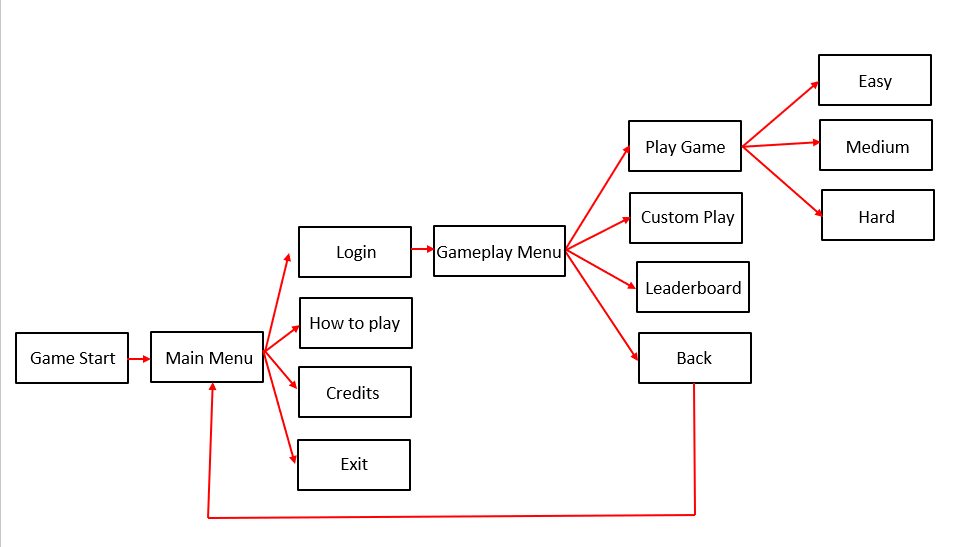
\includegraphics[scale=0.5]{Game Steps.png}\\[0.2cm]
    \textbf{Image 1.1.1: Game Steps}
\end{center}

\newpage
\section{Game Walkthroughs}
- When the user starts the game, at the main menu, they will have 4 options:\\
\indent\textbullet\textbf{ Login:} Enter gameplay.\\
\indent\textbullet\textbf{ How to play:} How to move, game rules and scoring methods in the game.\\
\indent\textbullet\textbf{ Credits:} How to move, game rules and scoring methods in the game.\\
\indent\textbullet\textbf{ Exit:} Exit the game.\\[0.2cm]
- Once the user selects \textbf{Login}, they will be redirected to the login interface and prompted to enter their email address in the correct format to proceed.\\
\hspace{-0.6cm}- Next, the user will be taken to the gameplay interface. Here, they will also be provided with 4 options:\\
\indent\textbullet\textbf{ Play Game:} User can choose 1 of 3 available modes:\\
\indent\indent- Easy: ...\\
\indent\indent- Medium: ...\\
\indent\indent- Hard: ...\\
\indent\textbullet\textbf{ Custom Play:} Users can set up their own game board by entering the size of rows and columns, and choosing whether they want their board to be automatically shuffled after each move or not.\\
\indent\textbullet\textbf{ Leaderboard:} Users can view the results of the top 5 players with the highest scores achieved so far.\\
\indent\textbullet\textbf{ Back:} Return to the main menu.\\[0.2cm]

\hspace{-0.6cm}\textbf{\underline{*GAME RULES:}}\\[0.2cm]
- Both "Play Game" and "Custom" gameplay are based on the same classic pattern.\\
- Gameplay consists of a board containing multiple cells representing characters or letters.\\
- The objective of the player is to select two cells with matching characters or letters that can be connected by 1 of 4 patterns: I, L, U, and Z.\\
- Validly connected patterns will make the two cells disappear.\\
- The game will end if the player clears all the cells on the board or runs out of 5 lives.\\
\begin{center}
    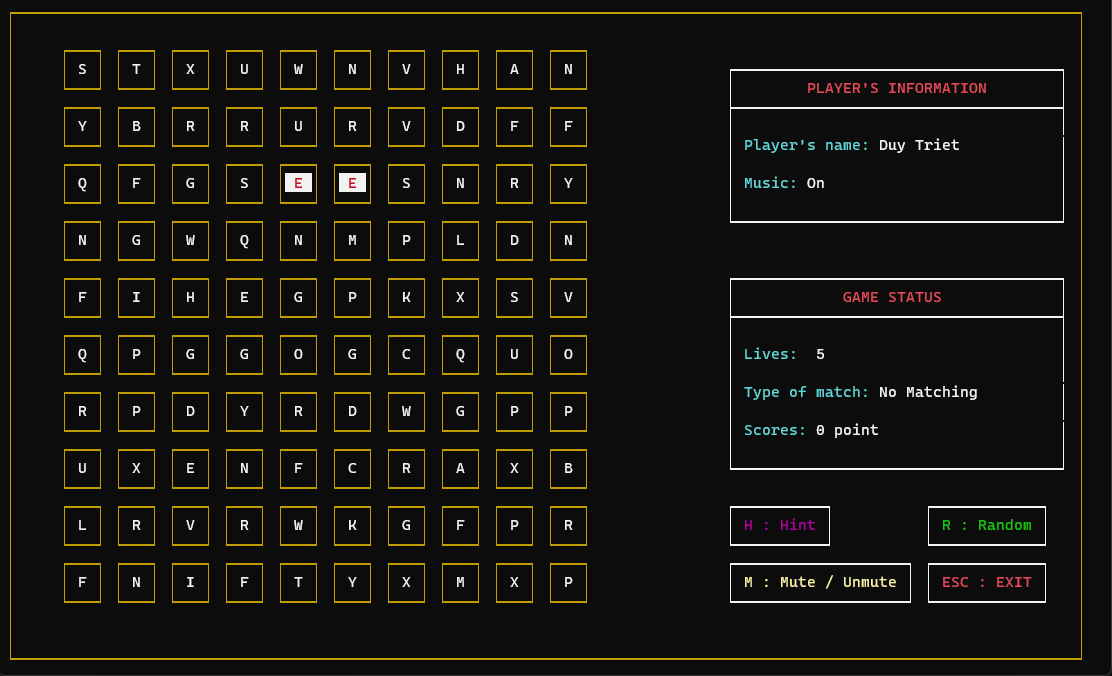
\includegraphics[scale=0.3]{Select.png}\\[0.2cm]
    \textbf{Image 1.2.1: Gameplay Interface}
\end{center}

\newpage
\chapter{FUNCTION}
\textbf{\large- How we organize files in the project.\\[0.2cm]
- Explain how the functions work.\\[0.2cm]
- List all the libraries and built-in functions we used in our project.}
\newpage
\section{File Structure}
The source code of the project is divided in total into 8 .cpp files and 8 header files.\\
Each file includes functions to perform tasks as its given filename\\[0.4cm]
\hspace{-0.6cm}\textbf{\underline{1/ Menu.cpp:}}\\[0.2cm]
- This file contains functions to generate complete interfaces and link them together with game files in this project.\\
- We have implemented the following function: \hl{void MainMenu();}\\
$\rightarrow$ This is the main function that will handle the entire main menu interface. It includes functions for printing animated text, displaying images, and processing the options selected by the user in this interface.
\begin{center}
    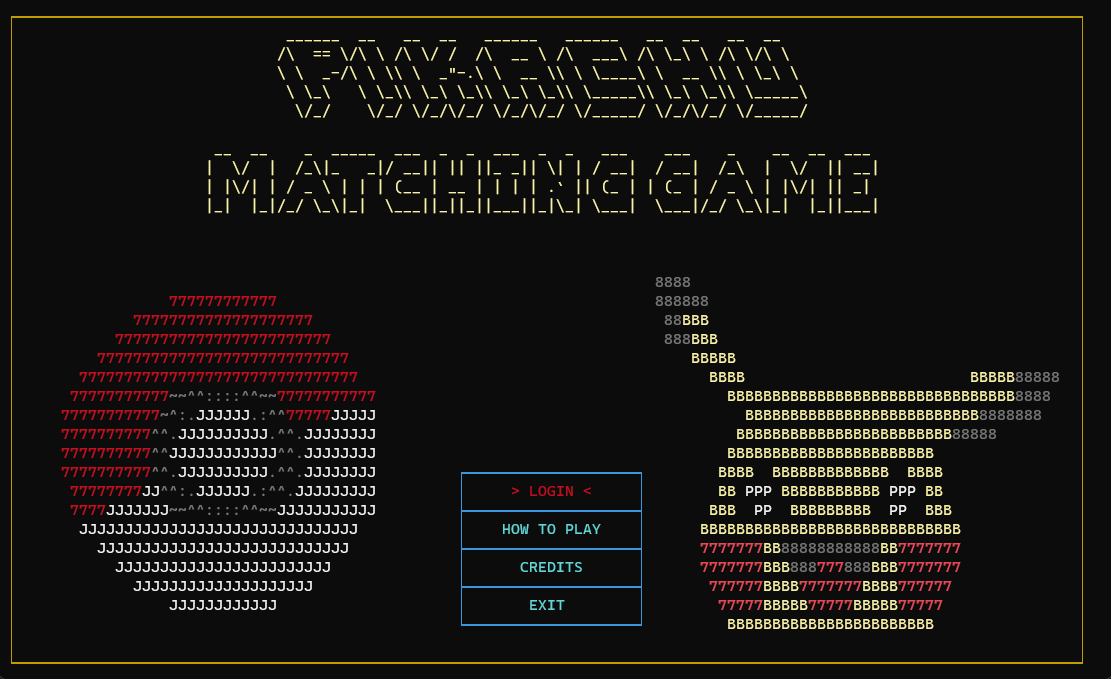
\includegraphics[scale=0.3]{Main Menu.png}\\[0.2cm]
    Image 2.1.1: Game starting
\end{center}
* Below, we will provide a more detailed explanation of the structure of this function:\\[0.2cm]
\hl{void \textbf{printMenu}(selection, x, y, w, h, textColor, buttonColor, backgroundColor, text);}\\
 $\rightarrow$ This is a sub-function in "MainMenu" function that defined some other functions for printing animated text and coloring images. These functions will be explained in detail in "Color effects" and "Visual effect" section later on.\\[0.2cm]
- The next step is to implement the method for highlighting the position of the option when the user uses arrow keys to navigate through the menu.\\
\hspace{-0.6cm}$\rightarrow$ We use a loop to get the user's input character and an integer variable called "selection" initialized with a value of 1. When the user presses the 'W' key (move up), the "selection" variable will be incremented by 1, and it will be decremented by 1 if the user presses the 'S' key (move down). Since the main menu only has 4 options, when the "selection" variable is 0, it will be reassigned to 4, and when it is 5, it will be set back to 1.\\[0.2cm]
- The "selectionMenu" is a subfunction within the "printMenu" function that handles the information about the position of the selected option by the user:\\
*\hl{void selectionMenu(int selection, int x, int y, int w, int h, int textColor, int buttonColor, int backgroundColor, string text);}\\
 $\rightarrow$ The task of the "selectionMenu" function is to change the text color of the first option to \textcolor{red}{red} when the "selection" variable has a value of 1, while keeping the text color of the other options as \textcolor{cyan}{cyan}. Similarly, it will change the text color of the second, third, or fourth option to \textcolor{red}{red} when the "selection" variable has a value of 2, 3, or 4, respectively.\\
$\rightarrow$ This simulates a cursor moving along the menu options based on the directional keys input by the user.\\[0.2cm]
- Based on the value of the selection variable, the switch-case statement will be used to determine which option the user has selected when they press the "Enter" key. Each case in the switch statement contains the corresponding commands to execute the selected option of the program.\\
- Two other sub-functions void LoginMenu(); (to generate menu interface after successful login) and void GamePlayMenu(); (menu for selecting the gameplay mode) also rely on a similar algorithm as in the MainMenu function to execute.\\[0.4cm]
\textbf{\underline{2/ User.cpp:}}\\[0.2cm]
\textbf{1/ Main.cpp:}\\
- This is the main part of the program.\\
- Header file included: \textbf{Menu.h}.\\[0.4cm]
\textbf{2/ Setup.cpp:}\\
- In this file, we install functions to set up the interface of the game such as: drawBorder, button (create buttons with content inside), box (draw cells for the game board), createScreen, clearScreen...\\
- Besides, there are also other supporting utilities in setting up the user experience: SetWindowSize, SetScreenBufferSize, DisableCtrButton, ShowScrollbar, showCursor, moveCursor, disableMouseInput, consoleColor, TextColor...\\
- Header file included: \textbf{Setup.h}.\\[0.4cm]
\textbf{3/ User.cpp:}\\
- The functions for reading, saving, and processing user's information are defined in this file: verify (check the correctness of the email entered by the user.), comparePlayers, pushRecord, printLeaderboard. \\
- Header file included: \textbf{User.h}.\\[0.4cm]
\textbf{4/ Graphic.cpp:}\\
- This file contains definitions of functions for reading artistic letters from text files and custom functions for handling images that appear in the game: art\_at\_pos, read\_file\_at\_pos, pokemon\_ball, login\_icon...\\
- Header file included: \textbf{Graphic.h}.\\[0.4cm]
\textbf{5/ Check.cpp:}\\
- Here, we define functions to check matching pattern motifs of I, L, Z, U, function to check whether the user wins or not and function to suggest moves to the user: check\_I, check\_L, check\_Z, check\_U, checkGameWin, moveSuggestion,...\\
- Header file included: \textbf{Check.h}.\\[0.4cm]
\textbf{6/ Board.cpp:}\\
- This file includes all the functions that generate the game board, notify the users when they make a right move or not, and also suggest a move: Board::drawBox, createBoard, retreatBoard, trueMatch, wrongMatch, suggestMatch,...\\
- Header file included: \textbf{Board.h}.\\[0.4cm]
\newpage
\hspace{-0.6cm}\textbf{\underline{7/ Game.cpp:}}\\[0.2cm]
- The functions in the this file, which are synthesized from the functions in the Check.cpp and Board.cpp files, are used to set up a complete interface for gameplay. In addition, they also provide an interface for users to input their names and customize the game board: gameLoop, playerInformation, normalForm, customForm, normalGame, customGame.\\
- Header file included: \textbf{Game.h}.\\[0.4cm]


\newpage
\section{Library}
- Data structures used in this program are arrays (used to hold the value of the
cells), linked list and queue (used to find the path to two cells).\\[0.4cm]
\textbf{\underline {1/ Library:}}
\verb|<Window.h>|\\[0.2cm]
- HANDLE console = GetStdHandle(STD\_OUTPUT\_HANDLE);\\
- HANDLE console = GetStdHandle(STD\_OUTPUT\_HANDLE);\\
- HWND hWnd = GetConsoleWindow();\\
$\rightarrow$ Used to handle the cursor position on the screen.\\
$\rightarrow$ If not using this, it will be hard to control the position of the cursor.\\[0.2cm]
- void SetWindowSize(int width, int height);\\
- void SetScreenBufferSize(SHORT width, SHORT height);\\
$\rightarrow$ Used to change the size of the console.\\
$\rightarrow$ If not using this, there will be a bug when the board is too big compares to the
screen.\\[0.2cm]
- void moveCursor(int posX, int posY);\\
$\rightarrow$ Used to put cursor to a desired position.\\
$\rightarrow$ If not using this, we can’t set the cursor to the position that we want.\\[0.2cm]
- SetConsoleTextAttribute(hConsoleOutput, wAttributes);\\
$\rightarrow$ Used to print text and background in color.\\
$\rightarrow$ If not using this, there will be no color effect.\\[0.4cm]
\textbf{\underline {2/ Library:}}
\verb|<conio.h>|\\[0.2cm]
- \_getch()\\
$\rightarrow$ Used to get a character entered by the user.\\
$\rightarrow$ If not using this, the user will not be able to control the cursor using a key-board.\\[0.4cm]
\textbf{\underline {3/ Library:}}
\verb|<ctime>|\\[0.2cm]
- clock\_t\\
$\rightarrow$ Used to calculate the time.\\
$\rightarrow$ If not using this, we can’t count the time of a gameplay.\\[0.2cm]
- srand()\\
$\rightarrow$ Used to initialize random number generator.\\
$\rightarrow$ If not using this, we can’t randomize the board.\\

\chapter{FEATURES}
\section{STANDARD FEATURES}
\subsection{Game starting}

\newpage
\subsection{I, L, U, Z matching}
- When the user selects two cells correctly in 1 of the 4 connection patterns (I, L, U, or Z), the system will display the selected connection pattern on the screen.\\
\begin{center}
    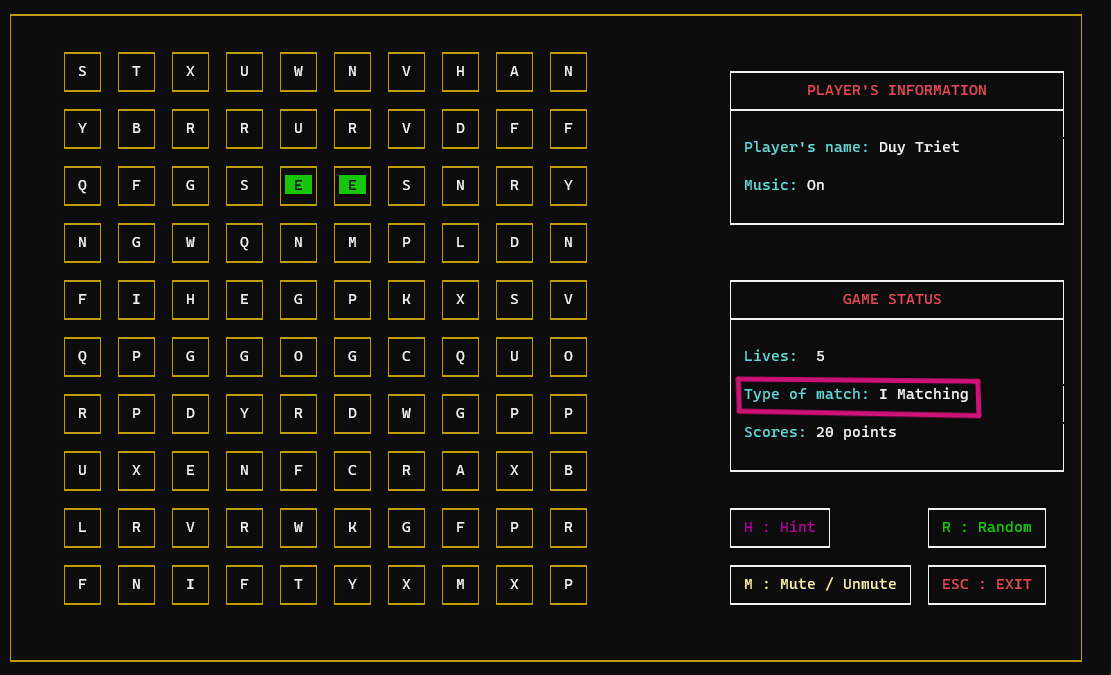
\includegraphics[scale=0.3]{Display matching pattern.png}\\[0.2cm]
    Image 3.1.2: Display matching pattern
\end{center}
\subsection{Game finish verify}
- When the user finishes a game level, the result will be displayed on the screen.\\
\begin{center}
    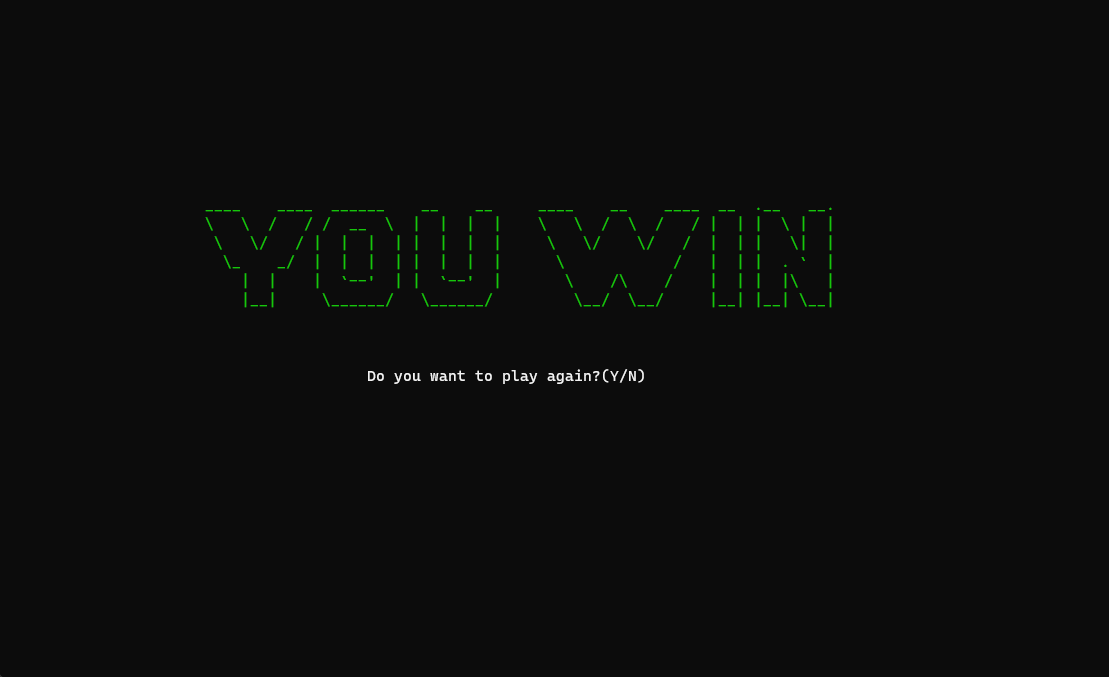
\includegraphics[scale=0.3]{You Win.png}\\
    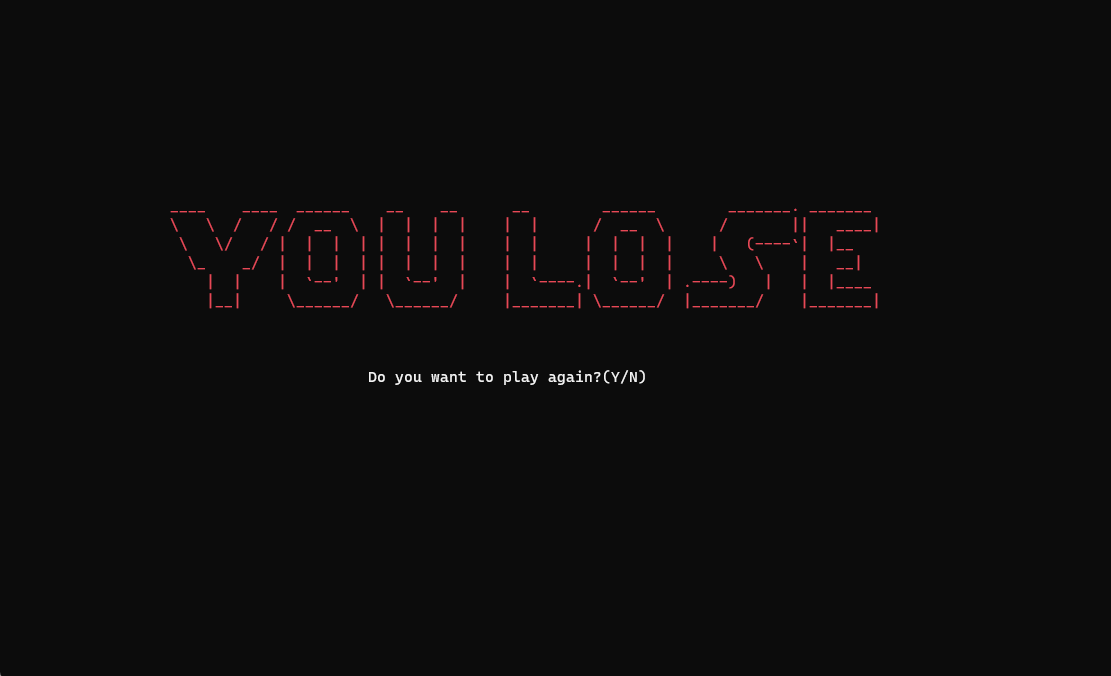
\includegraphics[scale=0.3]{You Lose.png}\\[0.2cm]
    Image 3.1.3: Game finish verify
\end{center}

\section{ADVANCED FEATURES}
\subsection{Color effects}
\textbf{- Interface:} Throughout all stages of the game, we have added various color effects to make it more visually appealing and enhance the overall user experience.
\begin{center}
    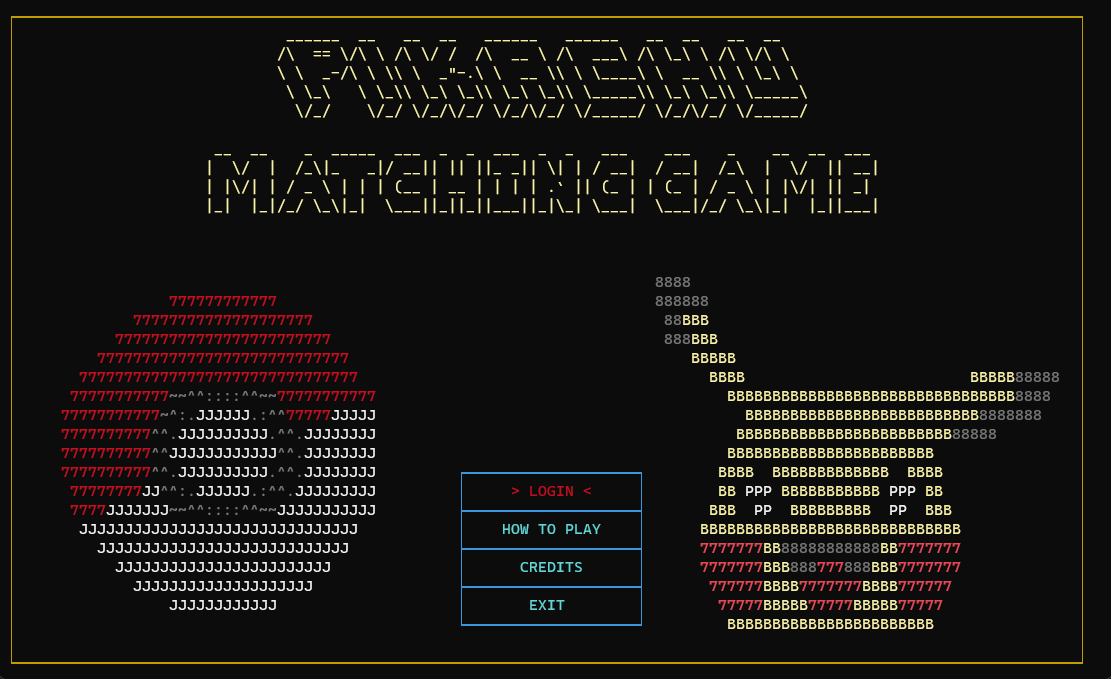
\includegraphics[scale=0.3]{Main Menu.png}\\[0.2cm]
    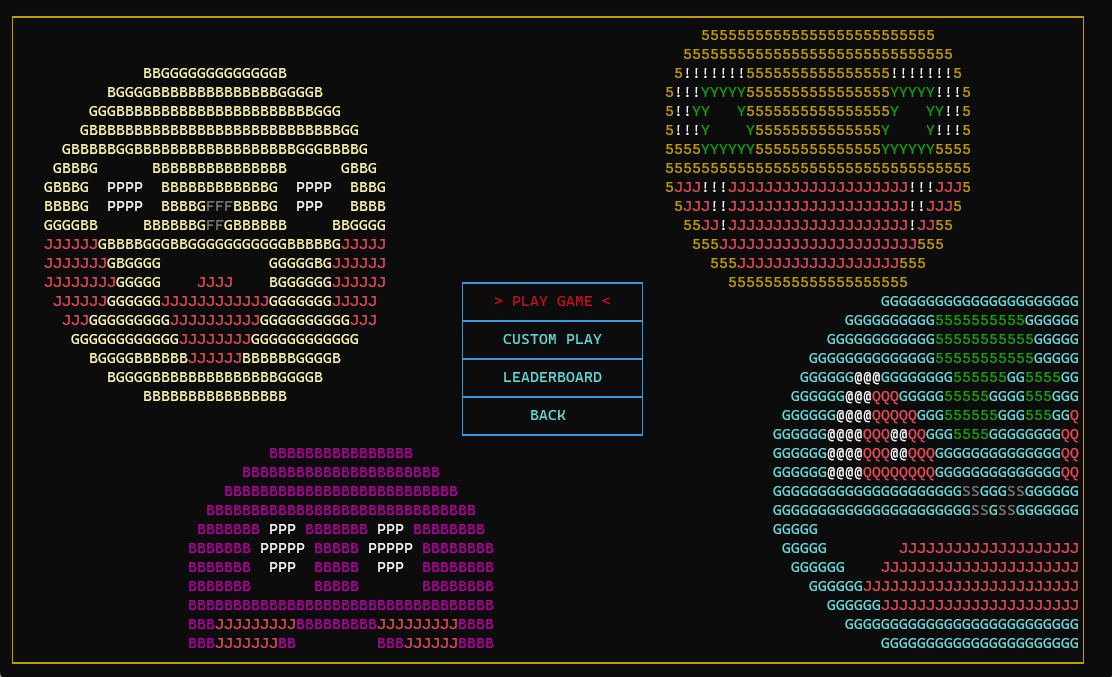
\includegraphics[scale=0.3]{Login Menu.png}\\[0.2cm]
    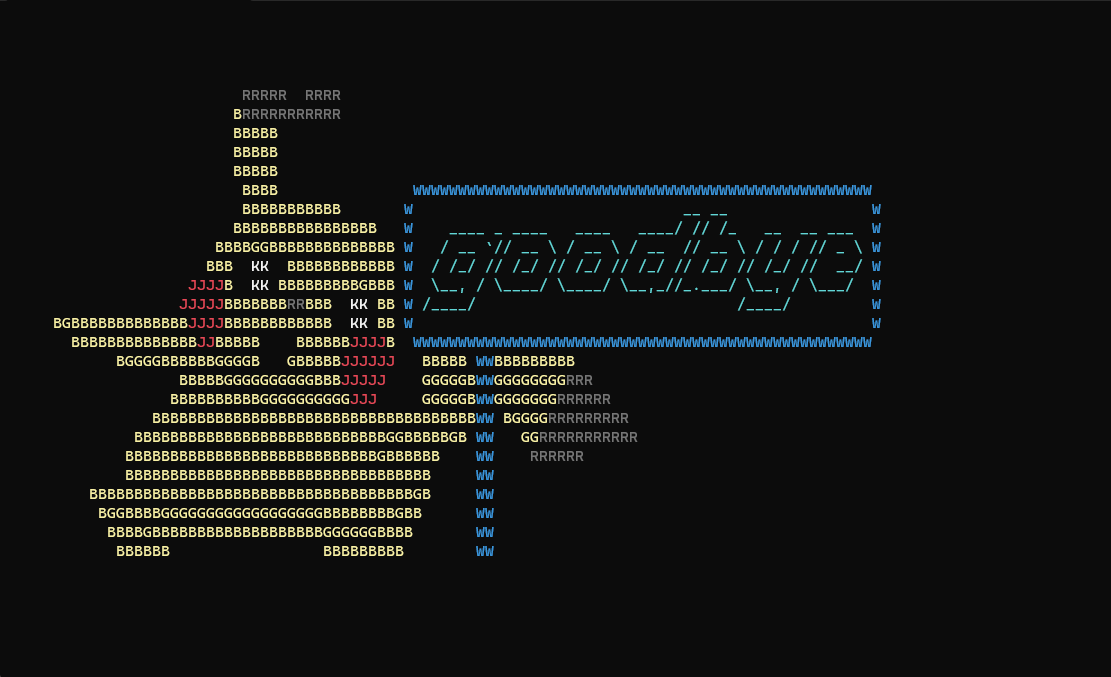
\includegraphics[scale=0.3]{Exit.png}\\[0.2cm]
    Image 3.2.1a: Color effects in interface
\end{center}
\newpage
\hspace{-0.6cm}\textbf{- Gameplay:} Color will appear in these 4 cases:\\[0.2cm]
. Selecting 2 cells $\rightarrow$ Light white.\\
. If 2 cells have the same value and a valid path $\rightarrow$ Green.\\
. If 2 cells don’t have the same value or a valid path $\rightarrow$ Red.\\
\begin{center}
    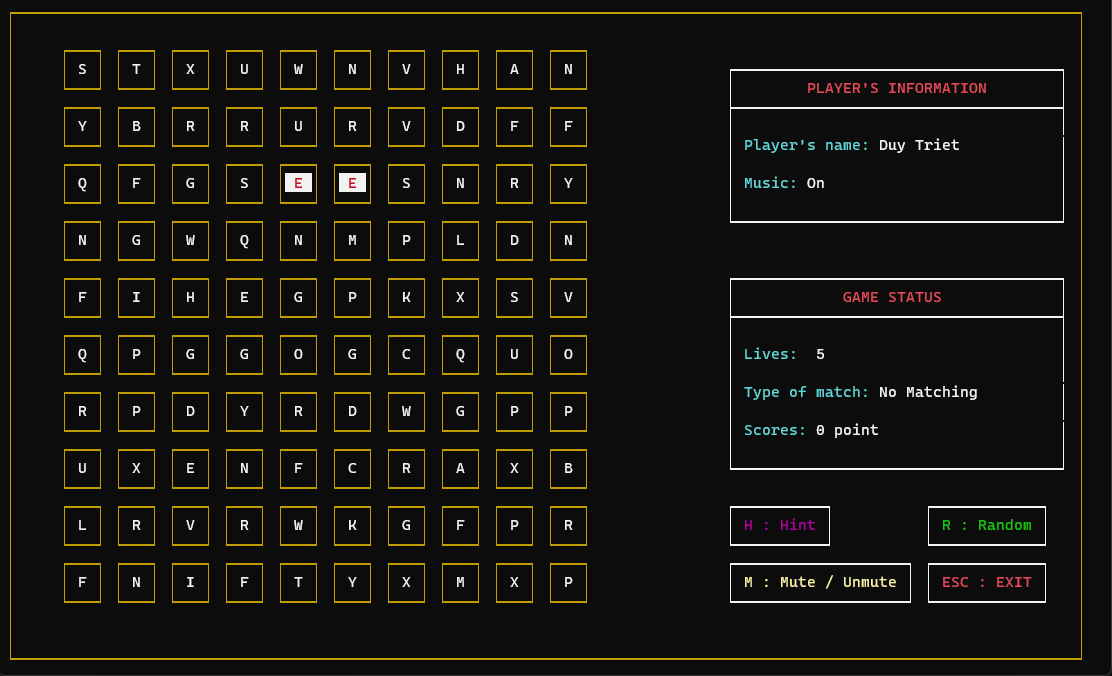
\includegraphics[scale=0.3]{Select.png}\\[0.2cm]
    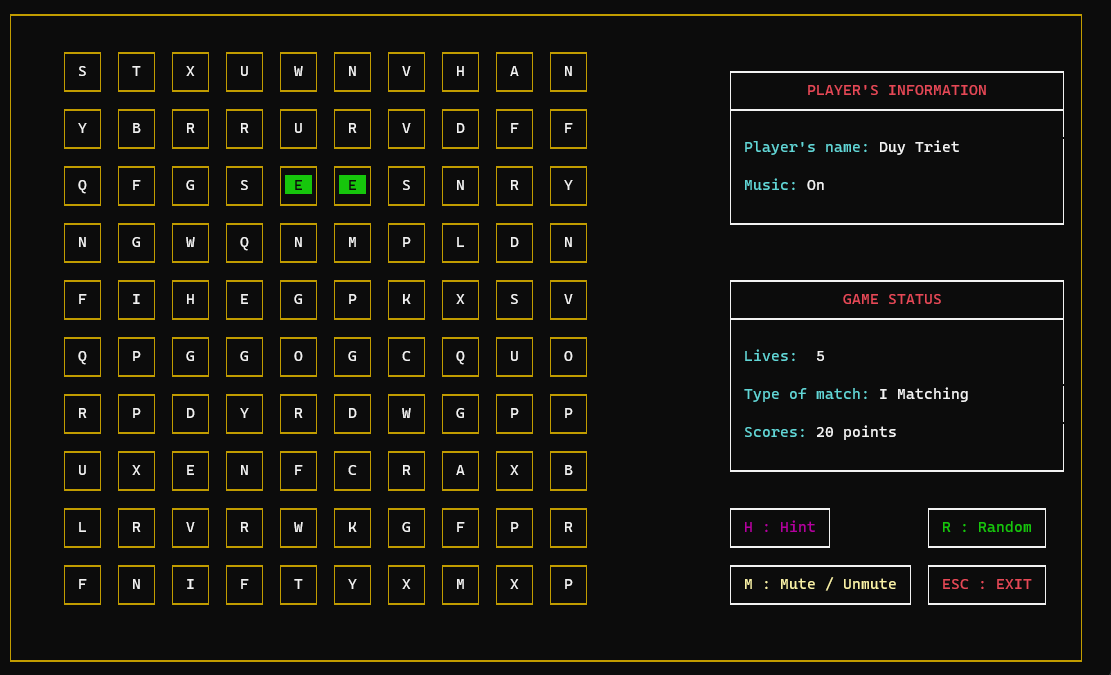
\includegraphics[scale=0.3]{Valid.png}\\[0.2cm]
    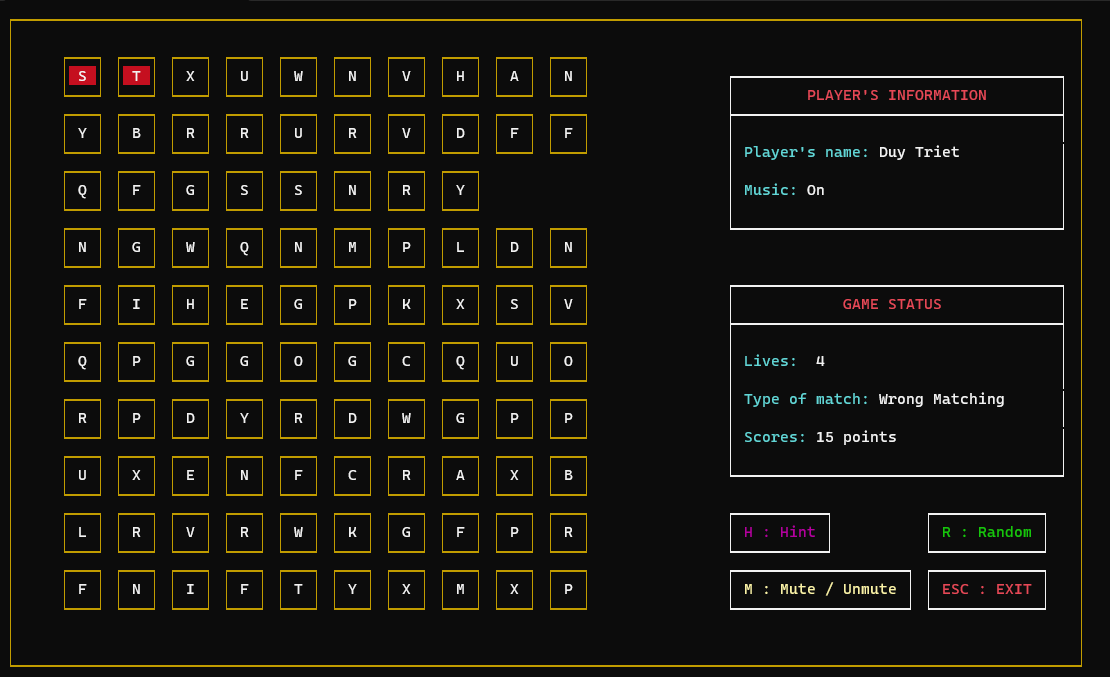
\includegraphics[scale=0.3]{Invalid.png}\\[0.2cm]
    Image 3.2.1b: Color effects in gameplay
\end{center}
\newpage
\subsection{Visual effects}
\begin{center}
    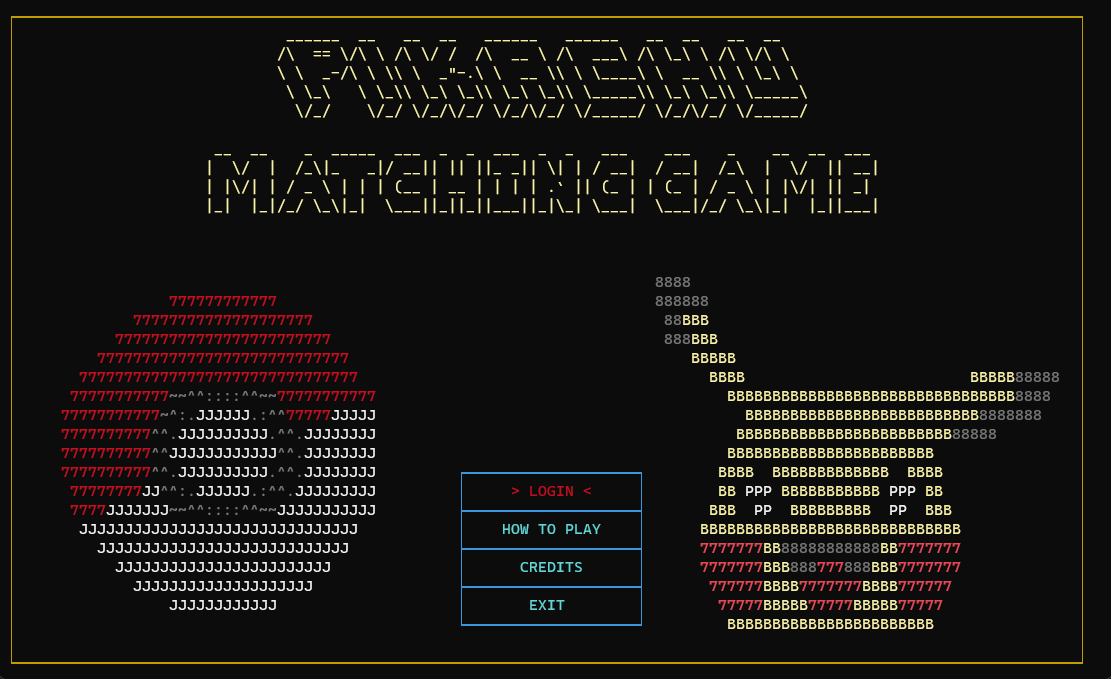
\includegraphics[scale=0.3]{Main Menu.png}\\[0.2cm]
    Image 3.2.2a: Main menu
\end{center}
\begin{center}
    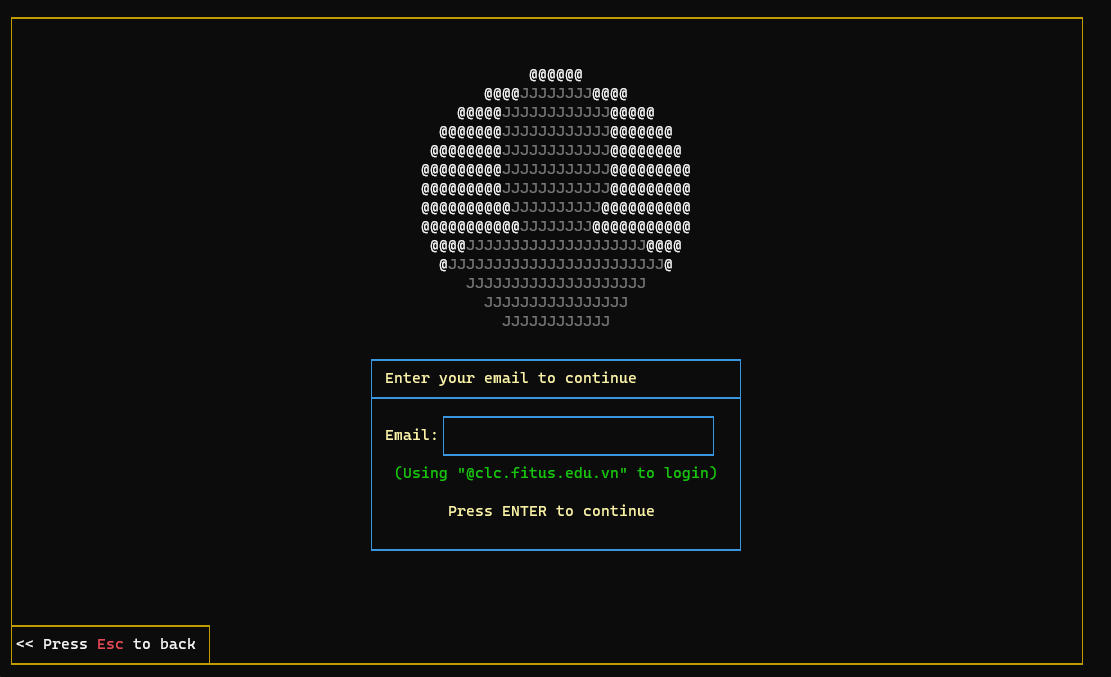
\includegraphics[scale=0.3]{Login Interface.png}\\[0.2cm]
    Image 3.2.2b: Login interface
\end{center}
\begin{center}
    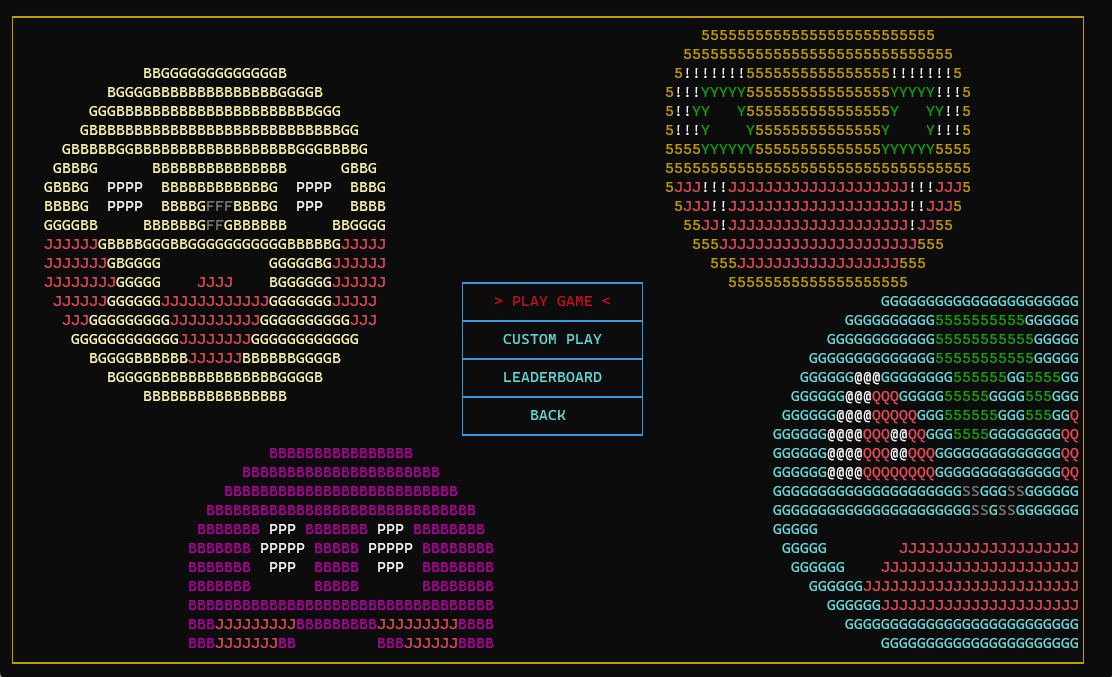
\includegraphics[scale=0.3]{Login Menu.png}\\[0.2cm]
    Image 3.2.2c: Login Menu
\end{center}
\begin{center}
    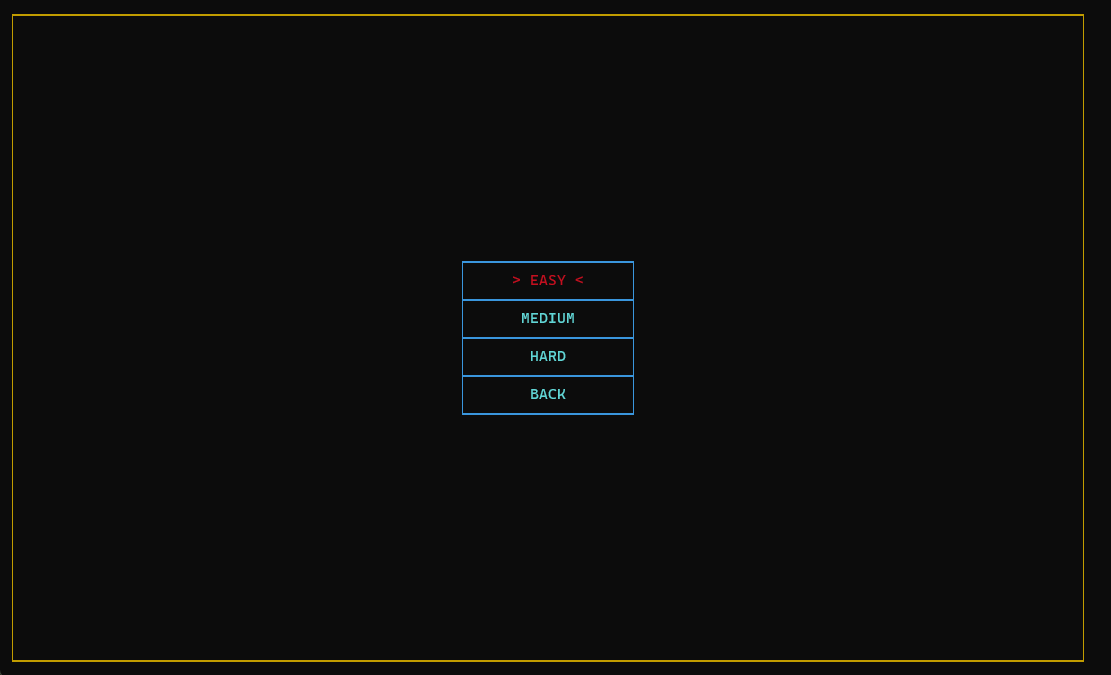
\includegraphics[scale=0.3]{Gameplay Modes.png}\\[0.2cm]
    Image 3.2.2d: Gameplay modes
\end{center}
\begin{center}
    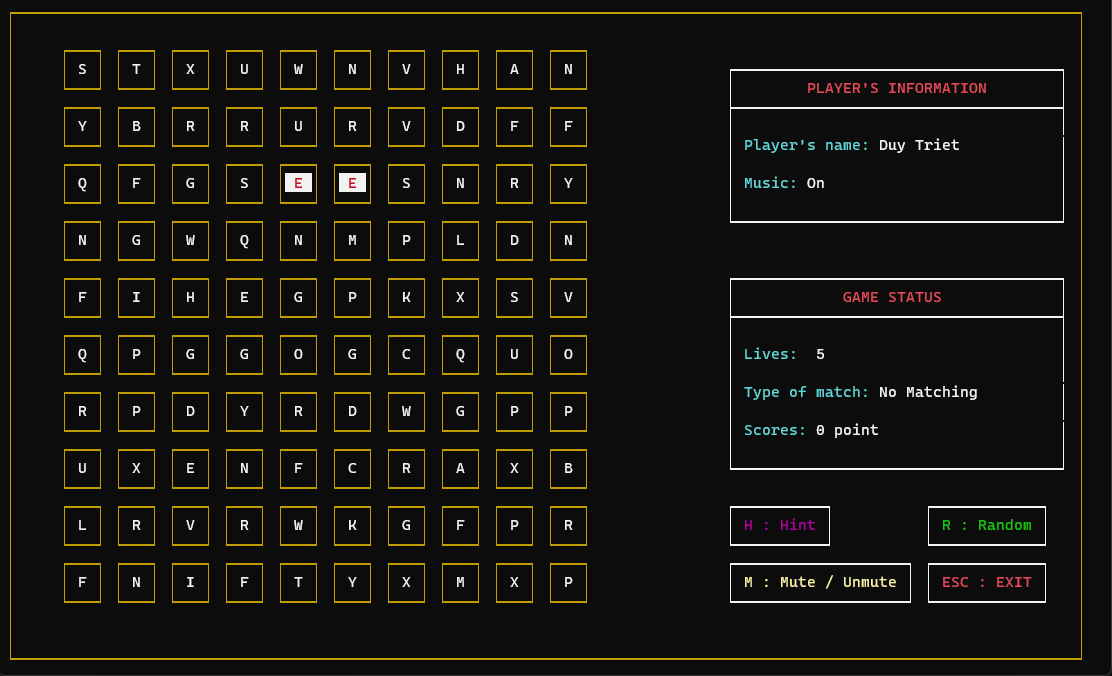
\includegraphics[scale=0.3]{Select.png}\\[0.2cm]
    Image 3.2.2e: Gameplay
\end{center}
\begin{center}
    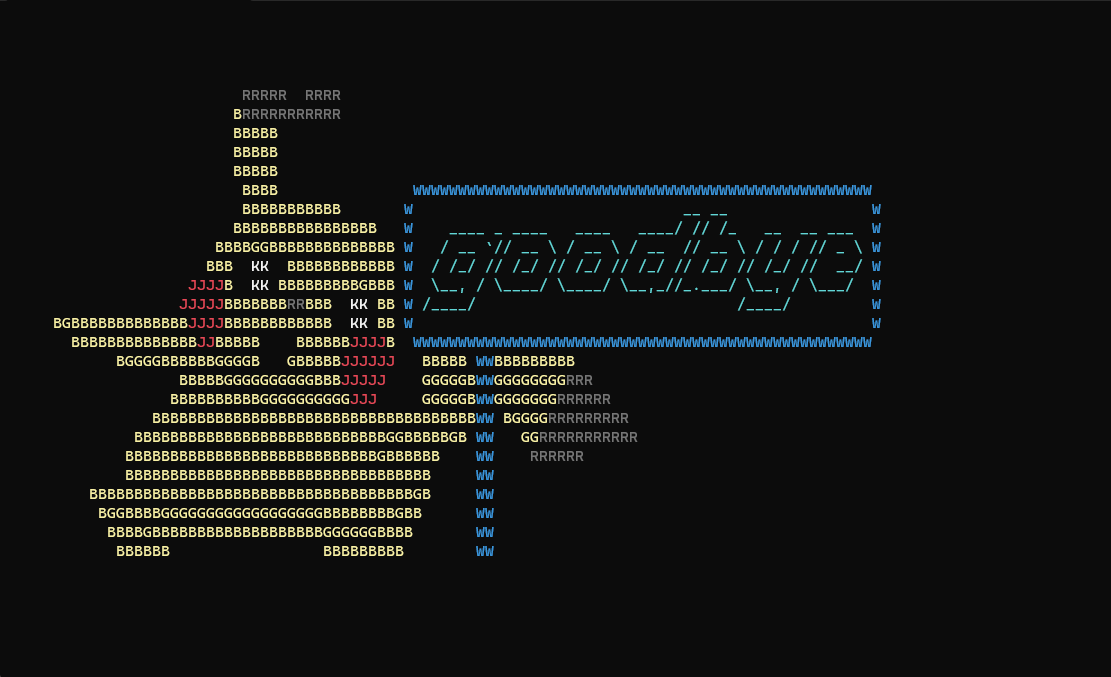
\includegraphics[scale=0.3]{Exit.png}\\[0.2cm]
    Image 3.2.2f: Exit
\end{center}
\newpage
\subsection{Sound effects}
\indent We mainly use this code to play music: 
\hl{PlaySound(TEXT("path"), NULL, SND\_ASYNC);}\\
$\rightarrow$ To make the code run on Windows, we include the "-lwinmm" flag in the execution command.
\subsection{Leaderboard}
- The top 5 players, who have achieved the highest scores and completed their games in the shortest time, will have their information registered on the Leaderboard.\\
- Here is how we implement this feature:\\
\indent {In file: User.cpp}\\
\indent {Function:}
\hl{bool comparePlayers(const Players \&p1, const Players \&p2);} \\
\indent - This function compares two players based on their points. If one player has higher points than the other, they will be swapped so that the player with higher points appears in front. If the points are equal, the player with shorter time will be considered. \\
\\
\indent {Function:}
\hl{long long unsigned int fileSize(string file);}\\
\indent - This function uses fseek() and ftell() to find the total size of the binary file in bytes, so that we can calculate the number of players in the binary file by dividing the size of the file by the size of the struct Players.\\
\\
\indent {Function:}
\hl{void pushRecord(Players p);}\\
\indent - This function is use to record high scores in write to binary file. There are 2 cases:
\indent $\rightarrow$ There are fewer than 5 players in the binary file. We will open the binary file in append and binary mode to write a new player to the end of the file. Next, we will reopen the binary file in binary mode and use std::sort() from the algorithm library to sort the players. Finally, we will open the binary file again in binary mode and write to the file once more.\\
\indent $\rightarrow$ There are 5 players in the binary file. We will open the binary file to read the data of the 5 players. After that, we will check if the new player has a better result than the fifth player in the binary file. If yes, we will replace the fifth player with the new one. Finally, we will sort the 5 players and write them back to the binary file.\\

\indent {Function:}
\hl{void printLeaderboard();}\\
\indent - This function is used to print the top 5 players by reading the datas from a binary file into a struct.
 
\begin{center}
    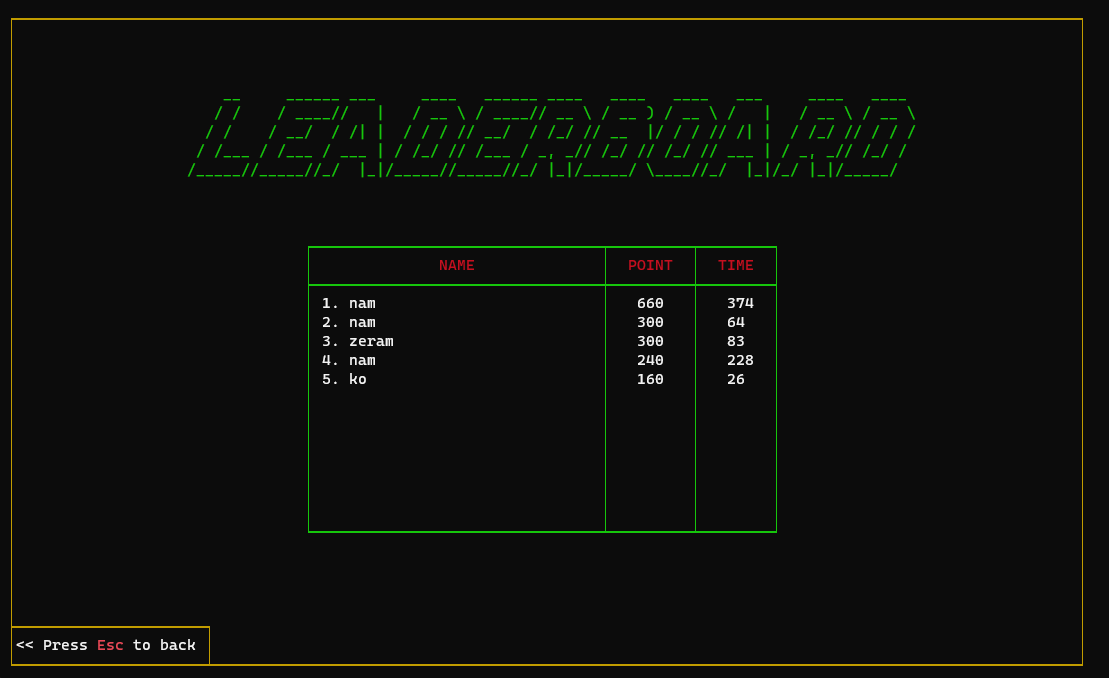
\includegraphics[scale=0.3]{Leaderboard.png}\\[0.2cm]
    Image 3.2.4: Leaderboard
\end{center}
\subsection{Move suggestion}
- When the "moveSuggestion" function is called by pressing "h" or "H", the hint will be shown in magenta background color in order to signal to the hint.\\
- Here is how we implement this feature:\\
\indent {In file: Check.cpp} \\
\indent {Function:}
\hl{bool moveSuggestion(Board **board, int \_row, int \_col, Point \&p1, Point \&p2);}\\
\indent - We will utilize 4 loops to identify valid pairs based on the boolean check provided by the function 
\hl{bool check\_All(Board **board, int \_row, int \_col, int x1, int y1, int x2, int y2);}. If the boolean check returns true, then there are valid pairs, which can be accessed by calling the 4 points p1.x, p1.y, p2.x, p2.y.
\begin{center}
    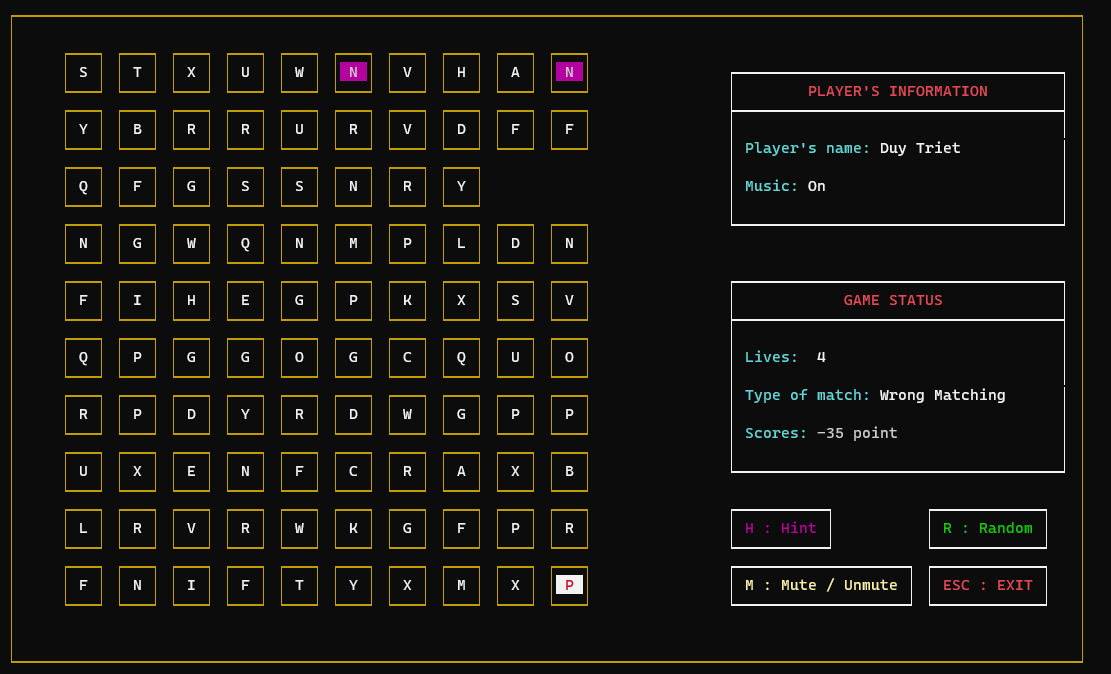
\includegraphics[scale=0.3]{Move Suggestion.png}\\[0.2cm]
    Image 3.2.5: Move suggestion
\end{center}
\section{OTHERS FEATURES}
\subsection{How to play}
\subsection{Auto shuffle if no valid pairs}
\chapter{REFERENCES}
{\textbf{\large All the resources that we have consulted for the project}}.\\[1.0cm]
1. Setup.cpp \\
\indent \textcolor{blue}{\href{https://learn.microsoft.com/en-us/cpp/?view=msvc-170}{https://learn.microsoft.com/en-us/cpp/?view=msvc-170}}\\[0.2cm]
\indent \textcolor{blue}{\href{https://stackoverflow.com/questions/2347770/how-do-you-clear-the-console-screen-in-c}{https://stackoverflow.com/questions/2347770/how-do-you-clear-the-console-screen-in-c}}\\[0.2cm]
\indent \textcolor{blue}{\href{https://cplusplus.com/forum/beginner/}{https://cplusplus.com/forum/beginner/}}\\[0.2cm]
\indent \textcolor{blue}{\href{https://codelearn.io/sharing/windowsh-va-ham-dinh-dang-console-p1}{https://codelearn.io/sharing/windowsh-va-ham-dinh-dang-console-p1}}\\[0.2cm]
\indent \textcolor{blue}{\href{https://codelearn.io/sharing/windowsh-ham-dinh-dang-noi-dung-console}{https://codelearn.io/sharing/windowsh-ham-dinh-dang-noi-dung-console}}\\[0.2cm]
2. Menu.cpp \\
\indent \textcolor{blue}{\href{https://cplusplus.com/forum/general/55170/}{https://cplusplus.com/forum/general/55170/}}\\[0.2cm]
\indent \textcolor{blue}{\href{https://www.youtube.com/watch?v=UjQIwlr_DqI}{https://www.youtube.com/watch?v=UjQIwlr\_DqI}}\\[0.2cm]
3. Check.cpp \\
\indent \textcolor{blue}{\href{https://cachhoc.net/2014/03/25/thuat-toan-game-pokemon-pikachu/}{https://cachhoc.net/2014/03/25/thuat-toan-game-pokemon-pikachu/}}\\[0.2cm]
4. Sounds we have use: \\
\indent \textcolor{blue}{\href{https://www.youtube.com/watch?v=RUCn4w-S2KM}{https://www.youtube.com/watch?v=RUCn4w-S2KM}}\\[0.2cm]
\indent \textcolor{blue}{\href{https://www.youtube.com/watch?v=jAIlKqL3nHo}{https://www.youtube.com/watch?v=jAIlKqL3nHo}}\\[0.2cm]
\indent \textcolor{blue}{\href{https://mixkit.co/free-sound-effects/tap/}{https://mixkit.co/free-sound-effects/tap/}}\\[0.2cm]
\indent \textcolor{blue}{\href{https://www.followchain.org/cristiano-ronaldo-siuuu-sound-effect/}{https://www.followchain.org/cristiano-ronaldo-siuuu-sound-effect/}}\\[0.2cm]
\indent \textcolor{blue}{\href{https://mixkit.co/free-sound-effects/game/}{https://mixkit.co/free-sound-effects/game/}}\\[0.2cm]

\end{document}
